\subsection{Q-Resolution Proof System}

In SAT solving, if a proposition is satisfiable, we can give a satisfying assignment, if it is unsatisfiable we will need to check every possible solution to be sure that the formula is not satisfiable, this is where a proof system comes in our help. For an unsatisfiable formula, we can give the steps in a proof system do derive a contradiction. One proof system for proposition formulas is the resolution proof system.

In QBF solving, we can elaborate a quantified version for the prior resolution proof system. This is presented in figure \ref{pre:qres}. Q-resolution proof system is refutational-complete for QBFs in PCNF, \cite{handbook}, this means if a formula is unsatisfiable, we can derive the empty clause, $\bot$, by applying rules from our proof system given the formula.

\stodo{what about satisfiable formulas}

\begin{figure}[H]
\centering
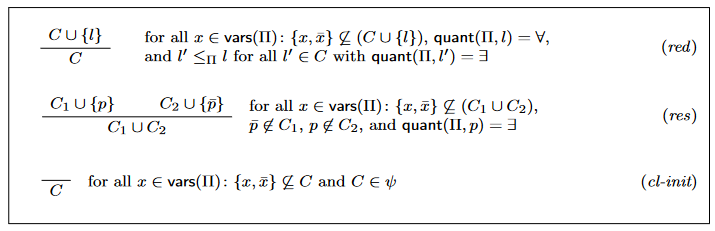
\includegraphics[width=1\textwidth]{../graphics/q-res-proof.png}
\caption{Q-resolution proof system from \cite{handbook}.}
\label{pre:qres}
\end{figure}

\begin{example}
    $\exists y \forall x z \exists p (y \lor x \lor z) \land p$ by applying only (red) for $(y \lor x \lor z)$ we get $(y \lor x)$ because $l \leq_\Pi x$ and $p$ is not in the clause, also we can get $(y \lor z)$ because $z$ needs to be higher than existential variables and ignore the universal quantified variables, in plus, if we apply it repeatedly we can also get $(y)$.
\end{example}

\textrosu{why tautology so probebatic}
\stodo{how to check sound of a red, with semantics?}

\begin{example}
    $\forall x y \exists z (x \lor z) \land (y \lor \overline{z})$ with (res) on those 2 clauses, we get $(x \lor y)$.
\end{example}

\begin{example}
    In this example we will apply the rules to get a refutation for $\forall x_1 x_2 \exists y (x_1 \lor x_2 \lor \overline{y}) \land (y \lor \overline{x_1}) \land (y \lor \overline{x_y}) \land y \land (x_1 \lor \overline{x_1})$. Firstly we apply (cl-init) where we get $(x_1 \lor x_2 \lor \overline{y}) \land (y \lor \overline{x_1}) \land (y \lor \overline{x_y}) \land y$ without last clause because that is a tautology. On the first and last clause we can apply (res) and get $(x_1 \lor x_2)$. On $(x_1 \lor x_2)$ we apply twice (red) and get the empty clause, $\bot$. Thus, our formula is false and have a proof in Q-resolution proof system.
\end{example}